\section{Background}
\label{background}

We now briefly review the starting points of our work: the Linux kernel
development model, the Linux backports project and the Coccinelle program
transformation tool.

\subsection{The Linux kernel development model}

As illustrated in Figure \ref{devmodel}, the development of a Linux kernel
release is carried out in four phases: the merge window, the release
candidate evaluation, the major release, and the maintenance of a stable
kernel.  The merge window begins immediately after the previous major
release, and lasts for 1-2 weeks.  During this period, maintainers who have
accumulated new features and device drivers for their subsystems request
that Linus Torvalds collect and integrate their changes.  This period
culminates in the release of the first release candidate (rc1) making the
complete set of merged changes available for general testing.  The release
of rc1 initiates the release candidate evaluation period.  The purpose of
this phase is to find and fix regressions for new code merged since the
last major kernel release.  There may be 5-9 release candidates, one per
week.  New drivers may be integrated during the release candidate
evaluation period.  Next comes the major release, making public the new
version.  At this point, the merge window for the next release begins.  In
parallel with the merge window, and beyond, possibly for several years, the
current release is maintained as a stable version.  Stable releases only
contain critical bug fixes; they may never contain new features or
drivers. Bug fixes are always sent upstream first, and must be merged into
Linus Torvalds' tree before being cherry picked or ported to older
maintained stable releases.

\begin{figure}
\[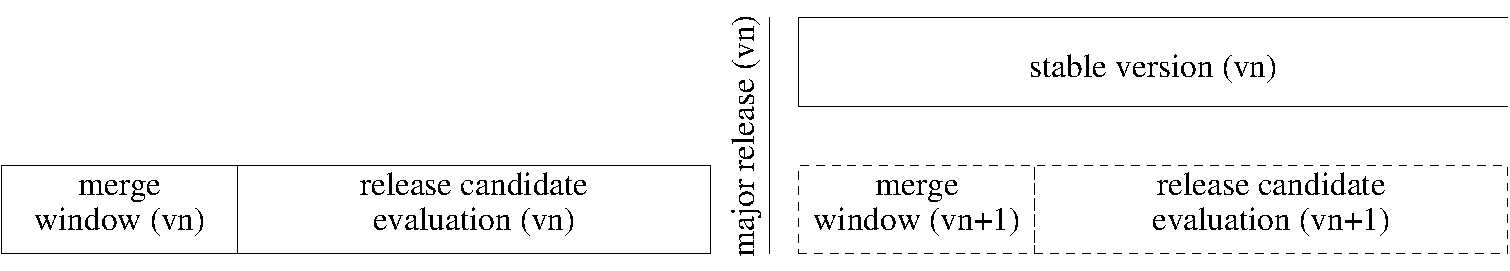
\includegraphics[width=\linewidth]{versions.pdf}\]
\caption{Four phases of Linux development}
\label{devmodel}
\end{figure}

The Linux kernel development model introduces some delay between when new
features are developed and when they are integrated into a release
candidate or major release.  To compensate for this delay, the
linux-next\footnote{git://git.kernel.org/pub/scm/linux/kernel/git/next/linux-next.git}
tree is used to mimic the merge window on daily basis, by pulling from each
subsystem tree. Every day the tree is reset to the latest major
kernel release and then each subsystem tree is pulled. The linux-next tree
can thus be used to track the latest development efforts on all subsystems on a
daily basis.

\subsection{A brief history of the Linux kernel backports project}

The Linux kernel backports
project\footnote{https://backports.wiki.kernel.org} was started in 2007 by
Luis R. Rodriguez while at Rutgers University, originally to help backport
the 802.11 subsystem and a series of 802.11 device drivers to a series of
older kernel
releases.\footnote{git://git.kernel.org/pub/scm/linux/kernel/git/mcgrof/compat-wireless-2.6-old.git}
The project was originally referred to as {\em compat-wireless}, reflecting
the initial target.  Over the years, the project grew to support more
device drivers and subsystems. In April 2012, at the Linux Collaboration
summit in San Francisco it was decided to rebrand the project {\em
  compat-drivers}\footnote{git://git.kernel.org/pub/scm/linux/kernel/git/mcgrof/compat-drivers-old.git}
when the project was folded under the Linux Foundation backports working
group.\footnote{http://lists.linuxfoundation.org/pipermail/lf\_driver\_backport/2012-August/001075.html}
The project now spearheads the Linux kernel backports effort. The last
rebranding of the project happened in April 2013, when it took on the name
{\em backports}, to distinguish it from the Linux kernel compat layer,
which addresses 64-bit and 32-bit compatibility.  The backports project is
now led by three core developers: Hauke Mehrtens, Johannes Berg,
Luis Rodriguez; two co-maintainers: Hauke and Luis; and is developed
and supported by a series of contributors.  It backports the subsystems Ethernet,
Wireless, Bluetooth, NFC, ieee802154, Media, and Regulator.

%% v2.6.30 - v3.6 - compat-wireless
%% v3.7 - v3.9 - compat-drivers
%% v3.10 - on - backports

The current goal of the backports project is to backport a slew of device
drivers from the latest major kernel releases down to a series of supported
stable kernel releases, at a minimum those listed on the main kernel
website, {\tt kernel.org}.  Currently, 18 releases are supported.  The
project's master development branch always tracks linux-next, allowing it
to track all the development trees. This ensures that at the end of each
merge window, the state of the backports will be very close to the state of
the first release candidate.  At this point, the backports project creates
a further branch that tracks the progress of the new release over the
release candidate evaluation period, to the major release, and on to its
lifetime as a stable kernel.  The backports project thus makes three kinds
of backports available: those derived from linux-next, those derived from
the most recent release candidate if any, and those derived from recent
stable kernels.  A user may prefer a backport from a stable kernel to one
from linux-next or from a release candidate, if one is available for the
desired driver.

As shown in Figure \ref{num}, as of September 2014, the backports project
backports almost 800 drivers.  These are kept up to date with linux-next
and the recent stable kernels each day, and are guaranteed to at least
compile correctly. Ensuring this each day typically requires 2-6 iterations
of test, refinements, and compiles for all supported versions. For this
development, the backports project uses a 32-core system with 236 GiB of
RAM.  Code generation and compile tests are all run in memory. As measured
by GNU {\tt time}, a full compilation test of a release across all 18
supported kernel revisions takes approximately 22 minutes of real time, 744
minutes of user mode time and 83 minutes of kernel time.  When the
backports project began in 2007, it provided backporting support for
drivers down to v2.6.25, first released in 2008. In order to scale to a
wider range of drivers, however, the project now only supports kernels down
to at most Linux v3.0, first released in 2011. The original motivation
behind the project was to encourage silicon manufacturers to work upstream
on the Linux kernel while providing them a solution for backporting their
drivers automatically down to older releases.  The framework is designed
{\em only} for Linux upstream drivers; the associated license enforces that
proprietary drivers cannot and should not use this framework.

\begin{figure}
\[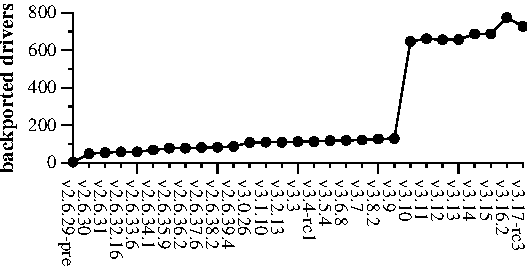
\includegraphics{supported.pdf}\]
\caption{Number of backported drivers, for kernels released since
  2009}
\label{num}
\end{figure}

\subsection{Coccinelle}

Coccinelle is a program matching and transformation engine for C code
\cite{Padioleau:eurosys08,Brunel:POPL09}.  It is released as open source,
and is available in a number of Linux distributions.  Coccinelle provides a
scripting language, SmPL ({\em semantic patch language}), that allows
patterns to be expressed as fragments of C code, and transformations to be
expressed by annotating lines of code with \verb+-+, for removal of the
matched code, or \verb-+-, for addition of the corresponding code.  As
such, SmPL specifications resemble {\em patches} \cite{diffmanual:02}.
Nevertheless, they are more robust than ordinary patches in that they are
insensitive to comments and whitespace, and take into account some aspects
of the code semantics such as control flow and type information.
Thus, we refer to SmPL specifications as {\em semantic patches}.

As a simple example of the use of Coccinelle, we consider the problem of
replacing all calls to a function named {\tt one} by calls to a function
named {\tt two}, and adding a {\tt NULL} argument.  The semantic patch that
makes this change is shown in Figure \ref{fig:sp1}.  This semantic patch
consists of a single rule that makes the complete transformation.  The rule
is in two parts: the declaration of {\em metavariables} that can match any
term of a specified type between the initial pair of {\tt @@} (lines 1-3),
followed by a {\em transformation specification} (lines 4-5).  In this
case, the only metavariable is {\tt arg}, which is declared to match any
expression.  The transformation specification then removes the call to {\tt
  one} with its argument, while at the same time binding the metavariable
{\tt arg} to this argument expression.  It then constructs a new function
call to the function {\tt two} with arguments the current binding of {\tt
  arg} and {\tt NULL}.  This semantic patch can be applied to an entire
code base.  A more detailed presentation of Coccinelle is available in
previous work \cite{Padioleau:eurosys08,Brunel:POPL09} and at the
Coccinelle website.\footnote{http://coccinelle.lip6.fr}

\begin{figure}
\begin{lstlisting}[language=diff]
@@
expression arg;
@@
- one(arg)
+ two(arg, NULL)
\end{lstlisting}
\caption{A simple semantic patch}
\label{fig:sp1}
\end{figure}

Coccinelle was originally motivated by a study of how the Linux kernel
evolves \cite{Padioleau:eurosys06}.  This study identified the problem of
{\em collateral evolutions}, in which the interface of a library changes,
and all clients of the library must be updated accordingly.  Coccinelle was
designed to help Linux developers make collateral evolutions faster and
more reliably.  The problem of implementing backports using Coccinelle is
related to the problem of collateral evolutions.  While collateral
evolutions were envisioned as being needed to modernize software, backports
must address changes in library interfaces to transport modern code to
older versions.

%% Furthermore, in practice even an aggressive
%% developer may only need to perform a collateral evolution infrequently,
%% perhaps once or twice a month. The use case for backports is very
%% different.  The code that has to be backported changes daily, via updates
%% in linux-next.  Thus, Coccinelle would have to be used daily, with all
%% semantic patches being applied against all supported subsystems and
%% drivers.

